% --------------------------------------------------------------
% This is all preamble stuff that you don't have to worry about.
% Head down to where it says "Start here"
% --------------------------------------------------------------
 
\documentclass[12pt]{article}
 
\usepackage[margin=1in]{geometry} 
\usepackage{amsmath,amsthm,amssymb}
\usepackage{mathtools}
\usepackage{multicol}
\usepackage{textcomp}
\usepackage{float}
\usepackage{longtable}

\newcommand{\N}{\mathbb{N}}
\newcommand{\Z}{\mathbb{Z}}
\newcommand\aug{\fboxsep=-\fboxrule\!\!\!\fbox{\strut}\!\!\!}
 
\newenvironment{theorem}[2][Theorem]{\begin{trivlist}
\item[\hskip \labelsep {\bfseries #1}\hskip \labelsep {\bfseries #2.}]}{\end{trivlist}}
\newenvironment{lemma}[2][Lemma]{\begin{trivlist}
\item[\hskip \labelsep {\bfseries #1}\hskip \labelsep {\bfseries #2.}]}{\end{trivlist}}
\newenvironment{exercise}[2][Exercise]{\begin{trivlist}
\item[\hskip \labelsep {\bfseries #1}\hskip \labelsep {\bfseries #2.}]}{\end{trivlist}}
\newenvironment{reflection}[2][Reflection]{\begin{trivlist}
\item[\hskip \labelsep {\bfseries #1}\hskip \labelsep {\bfseries #2.}]}{\end{trivlist}}
\newenvironment{proposition}[2][Proposition]{\begin{trivlist}
\item[\hskip \labelsep {\bfseries #1}\hskip \labelsep {\bfseries #2.}]}{\end{trivlist}}
\newenvironment{corollary}[2][Corollary]{\begin{trivlist}
\item[\hskip \labelsep {\bfseries #1}\hskip \labelsep {\bfseries #2.}]}{\end{trivlist}}
 
\begin{document}
 
% --------------------------------------------------------------
%                         Start here
% --------------------------------------------------------------
 
%\renewcommand{\qedsymbol}{\filledbox}
 

% --------------------------------------------------------------
%     You don't have to mess with anything below this line.
% --------------------------------------------------------------
% \documentclass[12pt]{article}

\usepackage[margin=1in]{geometry}
\usepackage{amsmath,amsthm,amssymb}
\usepackage{mathtools}
\usepackage{multicol}
\usepackage{textcomp}
\usepackage{float}
\usepackage{longtable}

\newcommand{\N}{\mathbb{N}}
\newcommand{\Z}{\mathbb{Z}}
\newcommand\aug{\fboxsep=-\fboxrule\!\!\!\fbox{\strut}\!\!\!}

\newenvironment{theorem}[2][Theorem]{\begin{trivlist}
\item[\hskip \labelsep {\bfseries #1}\hskip \labelsep {\bfseries #2.}]}{\end{trivlist}}
\newenvironment{lemma}[2][Lemma]{\begin{trivlist}
\item[\hskip \labelsep {\bfseries #1}\hskip \labelsep {\bfseries #2.}]}{\end{trivlist}}
\newenvironment{exercise}[2][Exercise]{\begin{trivlist}
\item[\hskip \labelsep {\bfseries #1}\hskip \labelsep {\bfseries #2.}]}{\end{trivlist}}
\newenvironment{reflection}[2][Reflection]{\begin{trivlist}
\item[\hskip \labelsep {\bfseries #1}\hskip \labelsep {\bfseries #2.}]}{\end{trivlist}}
\newenvironment{proposition}[2][Proposition]{\begin{trivlist}
\item[\hskip \labelsep {\bfseries #1}\hskip \labelsep {\bfseries #2.}]}{\end{trivlist}}
\newenvironment{corollary}[2][Corollary]{\begin{trivlist}
\item[\hskip \labelsep {\bfseries #1}\hskip \labelsep {\bfseries #2.}]}{\end{trivlist}}

\begin{document}

\title{TUTORIAL 1}%replace X with the appropriate number
\author{Timothée Guédon \& Tristan Glatard\\ %replace with your name
COMP 361 Numerical Methods} %if necessary, replace with your course title
\date{September 13, 2019}
\maketitle

\section{Exercises for today}

\begin{exercise}{1} %You can use theorem, proposition, exercise, or reflection here.
Classify the following matrices as singular, ill-conditioned, or well-conditioned using their determinant:\\
\begin{center}

%A
$\textbf{A}=
\begin{bmatrix}
1&2&3 \\4&5&6 \\ 7&8&9
\end{bmatrix}$
%B
$\textbf{B}=
\begin{bmatrix}
2&-2&1 \\1&0&-1 \\ 4&1&1
\end{bmatrix}$
%C
$\textbf{C}=
\begin{bmatrix}
1&2.0001&3 \\4&5&6 \\ 7&8&9
\end{bmatrix}$
\end{center}

\end{exercise}

\section{Bonus exercises}

You can try the following exercises at home for the next tutorial session.

\begin{exercise}{2} %You can use theorem, proposition, exercise, or reflection here.
Invert the following matrix using Gauss elimination or Gauss-Jordan elimination:
\begin{center}
\textbf{B}=
$\begin{bmatrix}
2&-2&1\\
1&0&-1\\
4&1&1
\end{bmatrix}
$
\end{center}
\end{exercise}

\begin{exercise}{3} %You can use theorem, proposition, exercise, or reflection here.
Invert the following matrix:
\begin{center}
\textbf{D}=
$\begin{bmatrix}
3&1&2\\
1&1&0\\
5&8&9
\end{bmatrix}
$
\end{center}
\end{exercise}

\break

\section{Solutions}

\subsection{Exercise 1}

They are two methods to find the condition of a matrix:
\begin{itemize}
  \item The formal measure of conditioning is the ``matrix condition number". It involves computing the norm of the matrix but also the norm of its inverse. If the condition number is close to 1 then the matrix is well conditioned.
  \item The second way of measuring the conditioning is the simpler one: By computing the determinant of the matrix and comparing it to the norm of the matrix. As it is a simpler method we shall start by computing it which will immediately show us if the matrix is singular or not.
\end{itemize}
Note that you can use the norm you want. You saw in the lecture the L1, L2 and infinity norms. You can use the one you want. \\

\textbf{First method: computing the determinant} \\

%Calculate det(A)
$
\vert A \vert = 1
\begin{vmatrix}
5&6 \\ 8&9
\end{vmatrix} - 2
\begin{vmatrix}
4&6 \\ 7&9
\end{vmatrix} + 3
\begin{vmatrix}
4&5 \\ 7&8
\end{vmatrix} = 45 - 48 - 2 (36-42) + 3 (32 - 35) = -3 + 2*6 - 3*3 = 0
$

\textit{A is singular.} \\

%Calculate det(B)
$
\vert B \vert = 2
\begin{vmatrix}
0&-1 \\ 1&1
\end{vmatrix} + 2
\begin{vmatrix}
1&-1 \\ 4&1
\end{vmatrix} + 1
\begin{vmatrix}
1&0\\4&1
\end{vmatrix}=2*1+2*5+1=13
$ \\

\textit{B is well-conditioned.} \\

%Calculate det(C)
$
\vert C \vert = 1
\begin{vmatrix}
5&6 \\ 8&9
\end{vmatrix} - 2.0001
\begin{vmatrix}
4&6 \\ 7&9
\end{vmatrix} + 3
\begin{vmatrix}
4&5 \\ 7&8
\end{vmatrix} = -3 + 2.0001*6 - 3*3 = 0.0006 \\
$ \\

Remember from the course that the determinant is considered small if it is smaller than the norm of the matrix (L1, L2, infinity). 0.0006 being close to zero we want to know if it can be considered ``ill conditioned". We will speak more about it in lab because this can be tricky. Let's try some norms for matrix C: \\

\textit{L1 norm}
$$
\| C \|_1 = \sum_{i=1}^n \sum_{j=1}^n { |A_{ij}^2| } = |1| + |2.0001| + |3| + |4| + ... + |9| = 45.0001
$$

\textit{L2 norm}
$$
\| C \|_2 = \sqrt { \sum_{i=1}^n \sum_{j=1}^n { A_{ij}^2 } } = \sqrt {1^2 + 2.0001^2 + ... + 9^2} = \sqrt {285.001} \approx 16.88
$$

\textit{Infinity norm}

$$\| C \|_\infty = \max_{1 \leq i \leq n}( { \sum_{j=1}^n { |A_{ij}| } })$$

\noindent $ = \max((|1| + |2.0001| + |3|), (|4| + |5| + |6|), (|7| + |8| + |9|))
\\ = \max (3*2 + 0.0001, 3*5, 3*8)
\\ = \max (6.0001, 15, 24)
\\ = 24
$

\hfill \break As $|C| << \| C \|$, C is ill-conditioned. Remember that $|C|$ is the determinant of C. \\

Although matrix $B$ seems well conditioned, we can verify it by comparing it to the norm of matrix $B$ too. Insure that you are able to find the following values for the norms of $B$:

$$\| B \|_1 = 13 $$

$$\| B \|_2 \approx 5.38$$

$$\| B \|_\infty = 6$$

We can see that $\| B \|$ is less than or equal to the determinant of $B$ Therefore, it confirms us that $B$ is well conditioned. \\

\textbf{Second method: computing the condition number} \\

Remember from the lecture that $cond(A)= \| A \| \| A^{-1} \| $. The condition number of matrix A cannot be computed because A is singular, and therefore non invertible. So let's start with matrix B. We will see in the next tutorial how to compute its inverse using Gauss elimination and Gauss-Jordan elimination. Today, let's just solve the system with the simple substitution method and compute the condition number of B: \\

Remember that inverting a matrix $B$ is equivalent to seeking $X = B^{-1}$, the inverse of matrix $B$ such that $BX=I$ (indeed, we know that $ BB^{-1} = I $) with $I$ being the identity matrix. We know how to solve a system with 3 unknowns for a given vector $b$. We can break the identity matrix $I$ into three vectors $b$:\\

$$ b = \begin{bmatrix}
  1 \\
  0 \\
  0
\end{bmatrix} b = \begin{bmatrix}
  0 \\
  1 \\
  0
\end{bmatrix} b = \begin{bmatrix}
  0 \\
  0 \\
  1
\end{bmatrix} $$

We want to solve following the system for each vector $b$ :
$$\begin{cases}
  2x - 2y + z = b_1 \\
  x - z = b_2 \\
  4x + y + z = b_3
\end{cases}$$

\textit{Solving for} $b = \begin{bmatrix}
  1 \\
  0 \\
  0
\end{bmatrix}$

$$\begin{cases}
  2x - 2y + z = 1 \\
  x - z = 0 \\
  4x + y + z = 0
\end{cases}$$

$$\begin{cases}
  2x - 2y + z = 1 \\
  x = z \\
  4x + y + z = 0
\end{cases}$$

$$\begin{cases}
  2x - 2y + z = 1 \\
  x = z \\
  y = -5z
\end{cases}$$

By solving equation 1 we get $z = \frac{1}{13} $ which gives us the values of $x$ and $y$ as well.

$$\begin{cases}
  x = \frac{1}{13} \\
  y = \frac{1}{13} \\
  z = \frac{-5}{13}
\end{cases}$$

\textit{Solving for} $b = \begin{bmatrix}
  0 \\
  1 \\
  0
\end{bmatrix}$

$$\begin{cases}
  2x - 2y + z = 0 \\
  x - z = 1 \\
  4x + y + z = 0
\end{cases}$$

$$\begin{cases}
  2x - 2y + z = 0 \\
  x = 1 + z \\
  4x + y + z = 0
\end{cases}$$

$$\begin{cases}
  2x - 2y + z = 0 \\
  x = 1 + z \\
  4(1 + z) + y + z = 0
\end{cases}$$

$$\begin{cases}
  2x - 2y + z = 0 \\
  x = 1 + z \\
  y = -4 -5z
\end{cases}$$

Again, by solving equation 1 we get $z = \frac{-10}{13} $ which gives us the values of $x$ and $y$ as well.

$$\begin{cases}
  x = \frac{3}{13} \\
  y = \frac{-2}{13} \\
  z = \frac{-10}{13}
\end{cases}$$

\textit{Solving for} $b = \begin{bmatrix}
  0 \\
  0 \\
  1
\end{bmatrix}$

$$\begin{cases}
  2x - 2y + z = 0 \\
  x - z = 0 \\
  4x + y + z = 1
\end{cases}$$

$$\begin{cases}
  2x - 2y + z = 0 \\
  x = z \\
  4x + y + z = 1
\end{cases}$$

$$\begin{cases}
  2x - 2y + z = 0 \\
  x = z \\
  y = 1 - 5z
\end{cases}$$

$$\begin{cases}
  x = \frac{2}{13} \\
  y = \frac{3}{13} \\
  z = \frac{2}{13}
\end{cases}$$

By combining the three vectors we found, we get the following inverse matrix:

$$ B^{-1} = \frac{1}{13} \begin{bmatrix}
  1 & 3 & 2 \\
  -5 & -2 & 3 \\
  1 & -10 & 2
\end{bmatrix}$$

We can verify that the solution is correct:

$$
BB^{-1} = \begin{bmatrix}
  2 & -2 & 1 \\
  1 & 0 & -1 \\
  4 & 1 & 1
\end{bmatrix}
\frac{1}{13} \begin{bmatrix}
  1 & 3 & 2 \\
  -5 & -2 & 3 \\
  1 & -10 & 2
\end{bmatrix}
= \frac{1}{13} \begin{bmatrix}
  13 & 0 & 0 \\
  0 & 13 & 0 \\
  0 & 0 & 13
\end{bmatrix}
= \begin{bmatrix}
  1 & 0 & 0 \\
  0 & 1 & 0 \\
  0 & 0 & 1
\end{bmatrix} = I
$$

Now than we have the inverse of $B$ we can compute its condition number using the norm we want, for example the infinity norm: \\
$ \| B \|_\infty = \max (5, 2, 6) = 6 $ \\
$ \| B^{-1} \|_\infty = \max (\frac{6}{13}, \frac{10}{13}, \frac{13}{13}) = \frac{13}{13} = 1 $ \\
$$ cond(B) = \| B \|_\infty  \| B^{-1} \|_\infty = 1.6 = 6 $$

We could do the exact same process on matrix $C$ to get $cond(C)$. You will find something like: \\
$$
C^{-1} = \begin{bmatrix}
  -5000 & 9998.5 & -4999 \\
  10000 & -20000 & 10000 \\
  -5000 & 10001.1667 & -5000.67
\end{bmatrix}
$$ \\

Resulting in $cond(C) = \| C \|_\infty  \| C^{-1} \|_\infty = 24 * 40,000 = 960,000$. As expected, $cond(C)$ is much greater than 1.

\end{document}
 
% % --------------------------------------------------------------
% This is all preamble stuff that you don't have to worry about.
% Head down to where it says "Start here"
% --------------------------------------------------------------
 

% --------------------------------------------------------------
%                         Start here
% --------------------------------------------------------------
 
%\renewcommand{\qedsymbol}{\filledbox}

\title{TUTORIAL 2}%replace X with the appropriate number
\author{TRISTAN GLATARD\\ %replace with your name
COMP 361 Numerial Methods} %if necessary, replace with your course title
\date{September 21, 2018} 
\maketitle

\begin{exercise}{1} %You can use theorem, proposition, exercise, or reflection here.  
Determine y at x = 0 using Lagrange\textquotesingle s method for the given data points:\\
\begin{table}[h]
\centering
\begin{tabular}{|c|c|c|c|}
\hline
x & -1.2 & 0.3 & 1.1 \\ \hline
y & -5.76 & -5.61 & -3.69 \\ \hline
\end{tabular}
\end{table}

\textbf{Solution.} With 3 given data points, we can construct a degree-2 polynomial using the Lagrange formula:\\
$$P_{2}(x)=\sum_{i=0}^2 y_{i}\ell_{i}(x)$$
where
\begin{align}
\ell_{0}(0)&=\frac{(x-x_1)(x-x_2)}{(x_0-x_1)(x_1-x_2)}=\frac{(0-0.3)(0-1.1)}{(-1.2-0.3)(-1.2-1.1)}&\approx 0.9565 \notag\\
\ell_{1}(0)&=\frac{(x-x_0)(x-x_2)}{(x_1-x_0)(x_1-x_2)}=\frac{(0+1.2)(0-1.1)}{(0.3+1.2)(0.3-1.1)}&= 1.1 \notag\\
\notag 
\ell_{2}(0)&=\frac{(x-x_0)(x-x_1)}{(x_2-x_0)(x_2-x_1)}=\frac{(0+1.2)(0-0.3)}{(1.1+1.2)(1.1-0.3)}&\approx -0.1956
\end{align}
Thus,
\begin{align}
\notag
y(0) = P_{2}(0) &=y_0\ell_0(0) + y_1\ell_2(0) + y_0\ell_2(0)\\ 
\notag
&\approx -5.76*0.9565 + (-5.61)*1.1+(-3.69)(-0.1956) 
\notag
\\&=-10.8726
\notag
\end{align}
\end{exercise}

%EXERCISE 2-----------------------------------------------------
\begin{exercise}{2} %You can use theorem, proposition, exercise, or reflection here.  
Use Newton\textquotesingle s method to find the polynomial that fits the following points:\\
\begin{table}[h]
\centering
\begin{tabular}{|c|c|c|c|c|c|}
\hline
x & -3 & 2 & -1 & 3 & 1 \\ \hline
y & 0 & 5 & -4 & 12 & 0 \\ \hline
\end{tabular}
\end{table}

\textbf{Solution.} Construct the tableau for Newton\textquotesingle s as follow

\begin{table}[H]
\centering
\begin{tabular}{|c|c|c|c|c|c|c|}
\hline
\textit{i} & $x_i$ & $y_i$ & $\nabla y_i$ & $\nabla ^2 y_i$ & $\nabla ^3 y_i$ & $\nabla ^4 y_i$ \\ \hline
0 & -3 & \textbf{0} &  &  &  &  \\ \hline
1 & 2 & 5 & \textbf{1} &  &  &  \\ \hline
2 & -1 & -4 & -2 & \textbf{1} &  &  \\ \hline
3 & 3 & 12 & 2 & 1 & \textbf{0} &  \\ \hline
4 & 1 & 0 & 0 & 1 & 0 & \textbf{0} \\ \hline
\end{tabular}
\end{table}

where elements are calculated as:\\
\begin{align}
\notag
\nabla y_1 &= \frac{y_1-y_0}{x_1-x_0}=\frac{5-0}{2+3}=1\\
\notag
\nabla y_2 &= \frac{y_2-y_0}{x_2-x_0}=\frac{-4+0}{-1+3}=-2\\
\notag
\nabla y_3 &= \frac{y_3-y_0}{x_3-x_0}=\frac{12-0}{3+3}=2\\
\notag
\nabla y_4 &= \frac{y_4-y_0}{x_4-x_0}=0\\
\notag
\nabla ^2 y_2 &= \frac{\nabla y_2-\nabla y_1}{x_2-x_1}=\frac{-2-1}{-1-2}=1\\
\notag
\nabla ^2 y_3 &= \frac{\nabla y_3-\nabla y_1}{x_3-x_1}=\frac{2-1}{3-2}=1\\
\notag
\nabla ^2 y_4 &= \frac{\nabla y_4-\nabla y_1}{x_4-x_1}=\frac{0-1}{1-2}=1\\
\notag
\nabla ^3 y_3 &= \frac{\nabla ^2 y_3-\nabla ^2 y_2}{x_3-x_2}=0\\
\notag
\nabla ^3 y_4 &= \frac{\nabla ^2 y_4-\nabla ^2 y_2}{x_4-x_2}=0\\
\notag
\nabla ^4 y_4 &= \frac{\nabla ^3 y_4-\nabla ^3 y_3}{x_4-x_3}=0\\
\notag
\end{align}
From the tableau \textquotesingle s diagonal, we have\\
\begin{align}
\notag
a_0&=y_0=0\\
\notag
a_1&=\nabla y_1=1\\
\notag
a_2&=\nabla ^2 y_2=1
\end{align}
and the polynomial fit is degree-2 (parabolic).
Evaluate backward with recurrence relations:
\begin{align}
\notag
P_0(x) &= a_2 = 1\\
\notag
P_1(x) &= a_1 + (x-x_1)P_0(x) = 1 + (x-2) = x-1\\
\notag
P_2(x) &= a_0 + (x-x_0)P_1(x) = 0 + (x+3)(x-1) = x^2+2x-3\\
\notag
\end{align}
\end{exercise}

%EXERCISE 2-----------------------------------------------------
\begin{exercise}{3} %You can use theorem, proposition, exercise, or reflection here.  
Use linear regression to find the line that fits the following data and determine the standard deviation:\\
\begin{table}[h]
\centering
\begin{tabular}{|c|c|c|c|c|c|}
\hline
x & -1.0 & -0.5 & 0 & 0.5 & 1.0 \\ \hline
y & -1.00 & -0.55 & 0.00 & 0.45 & 1.00 \\ \hline
\end{tabular}
\end{table}

\textbf{Solution.} With linear regression, we try to fit the data into a line of form
\begin{align}
f(x)=a+bx
\end{align}
where parameters a, b are given as
\begin{align}
b&=\frac{\sum\limits_{i=0}^{n} y_i(x_i-\overline{x})}{\sum\limits_{i=0}^{n} x_i(x_i-\overline{x})}\\
a&=\overline{y}-\overline{x}b
\end{align}

From the data:
\begin{align}
\notag
\overline{x}&=\frac{\sum\limits_{i=0}^{n} x_i}{n+1} = \frac{-1.0-0.5+0+0.5+1.0}{5} = 0 \\
\notag
\overline{y}&=\frac{\sum\limits_{i=0}^{n} y_i}{n+1}= \frac{-1.00 - 0.55 + 0.00 + 0.45 + 1.00}{5} = -0.02
\end{align}
Apply to (2) and (3)
\begin{align}
\notag
b&= \frac{(-1.00)(-1.0) + (-0.55)(-0.5) + 0.00*0 + 0.45*0.5 + 1.00*1.0}{(-1.0)(-1.0)+(-0.5)(-0.5)+0*0+0.5*0.5+1.0*1.0} = \frac{2.5}{2.5} = 1\\
\notag
a&=-0.02-0*1=-0.02
\end{align}
Then (1) becomes
\begin{align}
\notag
f(x)=-0.02 + x
\end{align}
We start the evaluation of the standard deviation by computing the residuals:
\begin{table}[h]
\centering
\begin{tabular}{|c|c|c|c|c|c|}
\hline
x & -1.0 & -0.5 & 0 & 0.5 & 1.0 \\ \hline
y & -1.00 & -0.55 & 0.00 & 0.45 & 1.00 \\ \hline
f(x) & -1.02 & -0.52 & -0.02 & 0.48 & 0.98 \\ \hline
y - f(x) & 0.02 & -0.03 & 0.02 & -0.03 & 0.02 \\ \hline
\end{tabular}
\end{table}
The sum of the squares of the residuals is
\begin{align}
\notag
S&=\sum\limits_{i=0}^4 [y_i-f(x_i)]^2\\
\notag
 &=(0.02)^2 + (-0.03)^2 + (0.02)^2 + (-0.03)^2 + (0.02)^2\\
 \notag
 &=0.003
\end{align}
The standard deviation is given as
\begin{align}
\notag
\sigma=\sqrt[]{\frac{S}{n-m}}
\end{align}
where $S$ is the sum of the squares of the residuals calculated above, $n + 1$ is the number of data points (i.e., $n = 4$), $m$ is the degree of the polynomial (1 in this case, since we fit linear regression)\\
Finally,
\begin{align}
\notag
\sigma=\sqrt[]{\frac{0.003}{4-1}} \approx 0.0316 
\end{align}
\end{exercise}
\begin{exercise}{4} %You can use theorem, proposition, exercise, or reflection here.  
Determine the natural cubic spline that passes through the data points:\\
\begin{table}[h]
\centering
\begin{tabular}{|c|c|c|c|}
\hline
x & 0 & 1 & 2 \\ \hline
y & 0 & 2 & 1 \\ \hline
\end{tabular}
\end{table}

Note that the interpolant consists of two cubics, one valid in $0 \leq x \leq 1$, the other in $1 \leq x \leq 2$. Verify that these cubics have the same first and second derivatives at $x = 1$.

\textbf{Solution.} With 3 given data points, we want to construct two cubics of the form:
\begin{align}
\notag
f_{0,1}(x) &= a_0x^3 + b_0x^2 + c_0x+d_0\\
\notag
f_{1,2}(x) &= a_1x^3 + b_1x^2 + c_1x+d_1
\end{align}

Interpolation gives us
\begin{align}
f_{0,1}(0) = 0 \Rightarrow d_0 = 0\\
f_{0,1}(1) = 2 \Rightarrow a_0 + b_0 + c_0 + d_0 = 2\\
f_{1,2}(1) = 2 \Rightarrow a_1 + b_1 + c_1 + d_1 = 2\\
f_{1,2}(2) = 1 \Rightarrow 8a_1 + 4b_1 + 2c_1 + d_1 = 1
\end{align}

The derivatives of these cubics are:
\begin{align}
\notag
f\prime_{0,1}(x) &= 3a_0x^2 + 2b_0x + c_0\\
\notag
f\prime_{1,2}(x) &= 3a_1x^2 + 2b_1x + c_1
\end{align}

The slope continuity condition gives us
\begin{align}
\notag
f\prime_{0,1}(1) &= f_{1,2}\prime(1)\\
3a_0 + 2b_0 + c_0 &= 3a_1 + 2b_1 + c_1
\end{align}

The second derivatives of these cubics are:
\begin{align}
\notag
f\prime\prime_{0,1}(x) &= 6a_0x + 2b_0\\
\notag
f\prime\prime_{1,2}(x) &= 6a_1x + 2b_1
\end{align}

The boundary conditions of natural spline give us
\begin{align}
f\prime\prime_{0,1}(0) &= 2b_0 = 0\\
f\prime\prime_{1,2}(2) &= 12a_1 + 2b_1 = 0
\end{align}

The continuity of second derivatives gives us
\begin{align}
\notag
f\prime\prime_{0,1}(1) &= f\prime\prime_{1,2}(1)\\
 6a_0 + 2b_0 &= 6a_1 + 2b_1
\end{align}

Solving the system of 8 equations with 8 unknowns gives us \\
$$a_0=-\frac{3}{4},b_0=0,c_0=\frac{11}{4},d_0=0$$\\
$$a_1=\frac{3}{4},b_1=-\frac{9}{2},c_1=\frac{29}{4},d_1=-\frac{3}{2}$$

It is easy to verify that $f\prime\prime_{0,1}(1) = f\prime\prime_{1,2}(1)$
\begin{align}
\notag
f\prime\prime_{0,1}(1) &= 6a_0 + 2b_0 = -\frac{9}{2}\\
\notag
f\prime\prime_{1,2}(1) &= 6a_1 + 2b_1 = -\frac{9}{2}
\end{align}

\textbf{Another solution (a shortcut)}

The three knots are equally spaced at h = 1. Recalling that the second
derivative of a natural spline is zero at the first and last knot, we have $k_0 = k_2 = 0$. 

The second derivatives at the second knot is obtained from Eq. (3.12) in the textbook:
$$k_{i-1}+4k_i+k_{i+1}=\frac{6}{h^2}(y_{i-1}-2y_i+y_{i+1}), i=1,2,...n-1$$

Using i = 1 results in
$$k_0+4k_1+k_2=6(y_0-2y_1+y_2)$$
$$k_1=-\frac{9}{2}$$

Now we can construct the cubics by applying Eq. (3.10) in the textbook:
\begin{align}
\notag
f_{i,i+1}(x) &= \frac{k_i}{6}\left[\frac{(x-x_{i+1})^3}{x_i-x_{i+1}}-(x-x_{i+1})(x_i-x_{i+1})\right]\\ 
\notag
& - \frac{k_{i+1}}{6}\left[\frac{(x-x_i)^3}{x_i-x_{i+1}}-(x-x_i)(x_i-x_{i+1})\right]\\ 
\notag
& + \frac{y_i(x-x_{i+1})-y_{i+1}(x-x_i)}{x_i-x_{i+1}}
\end{align}

With i=0,1 we have two cubics:
\begin{align}
\notag
f_{0,1}(x) &= - \frac{k_1}{6}\left[\frac{(x-x_0)^3}{x_0-x_1}-(x-x_0)(x_0-x_1)\right]
+ \frac{y_0(x-x_1)-y_1(x-x_0)}{x_0-x_1}\\
\notag
&=\frac{3}{4}\left[\frac{x^3}{0-1} - (x-1)(0-1)\right] - \frac{2x}{-1}\\
\notag
&= -\frac{3}{4}x^3 + \frac{11}{4}x\\ 
\notag
f_{1,2}(x) &=\frac{k_1}{6}\left[\frac{(x-x_2)^3}{x_1-x_2}-(x-x_2)(x_1-x_2)\right]
+\frac{y_1(x-x_2)-y_2(x-x_1)}{x_1-x_2}\\
\notag
&=-\frac{3}{4}\left[\frac{(x-2)^3}{1-2} - (x-2)(1-2)\right] - \frac{2(x-2)-(x-1)}{1-2}\\
\notag
&=\frac{3}{4}x^3-\frac{9}{2}x^2+\frac{29}{4}x-\frac{3}{2}
\end{align}
\end{exercise}


% --------------------------------------------------------------
%     You don't have to mess with anything below this line.
% --------------------------------------------------------------
 
\end{document}
 
% --------------------------------------------------------------
% This is all preamble stuff that you don't have to worry about.
% Head down to where it says "Start here"
% --------------------------------------------------------------
 

% --------------------------------------------------------------
%                         Start here
% --------------------------------------------------------------
 
%\renewcommand{\qedsymbol}{\filledbox}

\title{TUTORIAL 6}%replace X with the appropriate number
\author{TRISTAN GLATARD\\ %replace with your name
COMP 361 Numerial Methods} %if necessary, replace with your course title
\date{October 26, 2018} 
\maketitle

\begin{exercise}{1} %You can use theorem, proposition, exercise, or reflection here. 
Use the recursive trapezoidal rule to evaluate $ \int_0^{\frac{\pi}{4}} ln(1 + tan x)dx.$ Explain the results.

\textbf{Solution.} 

The recursive trapezoidal formulas for each iteration are:
Iteration 1:
\begin{align}
I_1=[f(a)+f(b)]\frac{H}{2} \notag
\end{align}
where 
\begin{align}
a&=0 \notag \\
b&=\frac{\pi}{4} \notag \\
H&=b-a=\frac{\pi}{4} \notag \\
\end{align}
Thus,
\begin{align}
I_1&=[ln(1+tan(0))+ln(1+tan(\frac{\pi}{4}))]\frac{\pi}{8} \notag \\
&\approx 0.2722 \notag
\end{align}
Iteration 2:
\begin{align}
I_2&=[f(a)+2f(a+\frac{H}{2})+f(b)]\frac{H}{4} \notag \\
&=[ln(1+tan(0))+2ln(1+tan(\frac{\pi}{8}))+ln(1+tan(\frac{\pi}{4}))]\frac{\pi}{16} \notag \\
&\approx 0.2722 \notag
\end{align}
Here we stop the iteration as $\vert I_2 - I_1\vert < \epsilon$.
This result means we only need one iteration for the recursive trapezoidal algorithm to converge. In other words, first approximation is already good enough.
This is intuitive if we look at the plot of f(x) = ln(1+tanx) on the interval \([0,\frac{\pi}{4}]\)

\textit{Hint: type \textbf{ln(1+tan(x))} on google search bar and it draws the plot for you.}

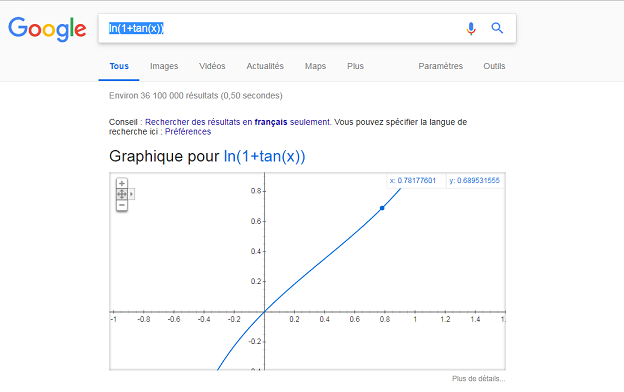
\includegraphics[]{plot_ln(1+tanx).png}

The plot looks very close to a line in that interval. Remember that with \textit{trapezoid} method, we approximate the function to a line so that the integral is approximated to the area of a trapezoid. That's why we have very close approximation right on first iteration.
\end{exercise}

%EXERCISE 2-----------------------------------------------------
\begin{exercise}{2} %You can use theorem, proposition, exercise, or reflection here.  
Evaluate $I=\int_{-1}^1 cos(2cos^{-1}x)dx$ with Simpson’s 1/3 rule using two, four, and six
panels. Explain the results.

\textbf{Solution.}

\textit{Note: just to make the notation clear, $cos^{-1}x$ denotes the arccosine function of \(x\) , not the power function.}

In this problem, \(a=-1, b=1\)

With two panels, let's denote $h= h_2=\frac{b-a}{2}=1$  we have three points at \([-1,0,1]\)

Then, the approximation using Simpson's 1/3 rule is
\begin{align}
I \approx I_2 &= \left[f(a) + 4f(\frac{a+b}{2}) + f(b)\right]\frac{h}{3} \notag \\
&=\left[cos(2*cos^{-1}(-1))+4cos(2*cos^{-1}(0)) + cos(2*cos^{-1}(1))\right]\frac{1}{3} \notag \\
&\approx -0.6666 \notag
\end{align}

With four panels, let's denote \(h= h_4=\frac{b-a}{4}=0.5\) we have two intervals to apply Simpson's 1/3 rule: three points at \([-1,-0.5,0]\) and another three points at \([0,0.5,1]\)
Then, the approximation using Simpson's 1/3 rule is
\begin{align}
I \approx I_4 &= \left[cos(2*cos^{-1}(-1))+4cos(2*cos^{-1}(-0.5)) + cos(2*cos^{-1}(0))\right]\frac{0.5}{3} \notag \\
&+ \left[cos(2*cos^{-1}(0))+4cos(2*cos^{-1}(0.5)) + cos(2*cos^{-1}(1))\right]\frac{0.5}{3} \notag \\
&\approx -0.6666 \notag
\end{align}

With six panels, let's denote \(h= h_6=\frac{b-a}{6}=0.3333\) we have three intervals to apply Simpson's 1/3 rule: three points at \([-1,-0.6666,-0.3333]\), \([-0.3333,0,0.3333]\) and another three points at \([0.3333,0.6666,1]\)
Then, the approximation using Simpson's 1/3 rule is
\begin{align}
I \approx I_6 &= \left[cos(2*cos^{-1}(-1))+4cos(2*cos^{-1}(-0.6666)) + cos(2*cos^{-1}(-0.3333))\right]\frac{0.3333}{3} \notag \\
&+ \left[cos(2*cos^{-1}(-0.3333))+4cos(2*cos^{-1}(0)) + cos(2*cos^{-1}(0.3333))\right]\frac{0.3333}{3} \notag \\
&+ \left[cos(2*cos^{-1}(0.3333))+4cos(2*cos^{-1}(0.6666)) + cos(2*cos^{-1}(1))\right]\frac{0.3333}{3} \notag \\
&\approx -0.6666 \notag
\end{align}
We can see that Simpson's rule seems to give the same approximation for two, four and six panels. 
Let's see how by looking at the plot of the function.

\textit{Hint: mathisfun.com has a cool widget that lets you approximate (and see plots) integrals of any functions of your choice.}

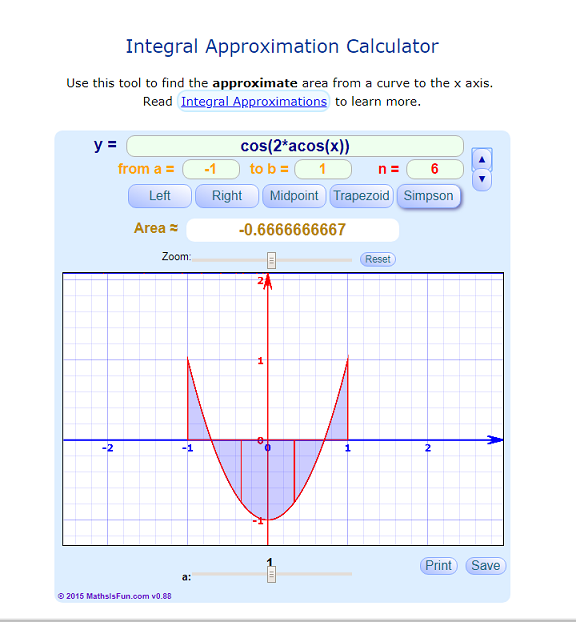
\includegraphics[]{cos(2acos(x)).png}


In the plot, we can the that the function \(cos(2*cos^{-1}(x))\) is a parabola. Remember that Simpson's 1/3 rule is derived from Newton-Cotes formulas with n = 2; that is, by passing a parabolic interpolant through three adjacent nodes. Because parabolic interpolation is unique with three points, we get exact results regardless of number of panels.
\end{exercise}


%EXERCISE 3-----------------------------------------------------
\begin{exercise}{3} %You can use theorem, proposition, exercise, or reflection here.  
The following table gives the pull F of the bow as a function of the draw x. If the bow is drawn 0.5m, determine the speed of the 0.075-kg arrow when it leaves the bow. Hint: The kinetic energy of the arrow equals the work done in drawing the bow; that is, $mv^2/2 = \int_0^{0.5m} Fdx$
\begin{table}[h]
\centering
\begin{tabular}{|c|c|c|c|c|c|c|c|c|c|c|c|}
\hline
x(m) &0.00& 0.05& 0.1& 0.15& 0.20 & 0.25&0.30&0.35&0.40&0.45&0.50\\ \hline
F(N)& 0& 37& 71 &104 &134 &161 &185& 207& 225& 239& 250 \\ \hline
\end{tabular}
\end{table}

\textbf{Solution.} 

In this problem, we have 11 evenly-spaced data points (or, 10 panels) with \(h=0.05\).
So we can approximate the integral  $\int_0^{0.5m} Fdx$ by applying Simpson's 1/3 rule on five pairs of panels:
On \([0,0.05,0.1]\)
 \begin{align}
 I_{0,0.1} &\approx \left[F(0) + 4F(0.05) + F(0.1)\right]\frac{0.05}{3} \notag \\
 &=(0+4*37+71)\frac{0.05}{3} = 3.65 \notag
 \end{align}
On \([0.1,0.15,0.2]\)
 \begin{align}
 I_{0.1,0.2} &\approx \left[F(0.1) + 4F(0.15) + F(0.2)\right]\frac{0.05}{3} \notag \\
 &=(71+4*104+134)\frac{0.05}{3} = 10.35 \notag
 \end{align}
On \([0.2,0.25,0.3]\)
 \begin{align}
 I_{0.2,0.3} &\approx \left[F(0.2) + 4F(0.25) + F(0.3)\right]\frac{0.05}{3} \notag \\
 &=(134+4*161+185)\frac{0.05}{3} = 16.05 \notag
 \end{align}
On \([0.3,0.35,0.4]\)
 \begin{align}
 I_{0.3,0.4} &\approx \left[F(0.3) + 4F(0.35) + F(0.4)\right]\frac{0.05}{3} \notag \\
 &=(185+4*207+225)\frac{0.05}{3} = 20.63 \notag
 \end{align}
On \([0.4,0.45,0.5]\)
 \begin{align}
 I_{0.4,0.5} &\approx \left[F(0.4) + 4F(0.45) + F(0.5)\right]\frac{0.05}{3} \notag \\
 &=(225+4*239+250)\frac{0.05}{3} = 23.85 \notag
 \end{align}
 Then,
 \begin{align}
 I=\sum I_{i,i+2}&= I_{0,0.1}+I_{0.1,0.2}+I_{0.2,0.3}+I_{0.3,0.4}+I_{0.4,0.5}\notag \\
 &\approx 3.65 + 10.65 + 16.05+20.63 + 23.85 \notag \\
 &=74.83 \notag
 \end{align}
 Now the speed of the arrow would be
 
 \begin{align}
 v&=\sqrt{\frac{2I}{m}} \notag \\
 &=\sqrt{\frac{2*74.83}{0.075}} \notag \\
 &\approx 44.67 \notag
 \end{align}
 \end{exercise}

\begin{exercise}{4} Evaluate $\int_1^\pi \frac{ln(x)}{x^2-2x+2}dx$
with Gauss-Legendre quadrature. Use (a) two nodes; and (b) four nodes.

\textbf{Solution}
First we need to "transform" the integration range \([1,\pi]\) to the one required by Gauss-Legendre quadrature \([-1,1]\).
\begin{align}
x&=\frac{b+a}{2} + \frac{b-a}{2}\xi \notag \\
&=\frac{\pi+1}{2} + \frac{\pi-1}{2}\xi \notag
\end{align}
\end{exercise}
Now \(dx = d\xi \frac{b-a}{2}\), and the quadrature becomes
\begin{align}
\int_1^\pi \frac{ln(x)}{x^2-2x+2}dx = \frac{\pi-1}{2} \sum_0^n A_if(x_i)
\end{align}
a) With two nodes, we have the following table of calculation (see Table 6.3 on Kiusalaas 2011)

\begin{table}[h]
\centering
\begin{tabular}{|r|r|r|r|r|}
\hline
\multicolumn{1}{|c|}{\textit{\textbf{\(\xi_i\)}}} & \multicolumn{1}{c|}{\textit{\textbf{\(x_i\)}}} & \multicolumn{1}{l|}{\textit{\(f(x_i\))}} & \multicolumn{1}{l|}{\textit{\(A_i\)}} & \multicolumn{1}{l|}{\textit{\(A_i*f(x_i)\)}} \\ \hline
-0.577350 & 1.452572 & 0.309868 & 1.000000 & 0.309868 \\ \hline
0.577350 & 2.689021 & 0.256743 & 1.000000 & 0.256743 \\ \hline
\end{tabular}
\caption{Abscissas and weights for Gauss-Legendre, n=1}
\label{tab-gauss-legendre-2-nodes}
\end{table}

Then we have approximation
\begin{align}
I&\approx\frac{\pi-1}{2} \sum_0^1 A_if(x_i) \notag \\
&=\frac{3.141593-1}{2} (0.309868+0.256743) \notag \\
&=0.606725 \notag
\end{align}
b) Now with four nodes, we have the following table of calculation

\begin{table}[h]
\centering
\begin{tabular}{|r|r|r|r|r|}
\hline
\multicolumn{1}{|c|}{\textit{\textbf{\(\xi_i\)}}} & \multicolumn{1}{c|}{\textit{\textbf{\(x_i\)}}} & \multicolumn{1}{l|}{\textit{\(f(x_i\))}} & \multicolumn{1}{l|}{\textit{\(A_i\)}} & \multicolumn{1}{l|}{\textit{\(A_i*f(x_i)\)}} \\ \hline
-0.339981 & 1.706746 & 0.356514 & 0.652145 & 0.232499 \\ \hline
-0.861136 & 1.148695 & 0.135628 & 0.347855 & 0.047179 \\ \hline
0.339981 & 2.434847 & 0.290927 & 0.652145 & 0.189727 \\ \hline
0.861136 & 2.992898 & 0.220499 & 0.347855 & 0.076702 \\ \hline\end{tabular}
\caption{Abscissas and weights for Gauss-Legendre, n=3}
\label{tab-gauss-legendre-4-nodes}
\end{table}
Then we have approximation
\begin{align}
I&\approx\frac{\pi-1}{2} \sum_0^3 A_if(x_i) \notag \\
&=\frac{3.141593-1}{2} (0.232499+0.047179+0.189727+0.076702) \notag \\
&=0.584768 \notag
\end{align}



% --------------------------------------------------------------
%     You don't have to mess with anything below this line.
% --------------------------------------------------------------
  
\end{document}
